% chapters/02_background.tex
\section{Tensor Networks}\label{sec:tensor-networks}

\subsection{Tensor Notation and Diagrams}\label{sec:tensor-notation}

\subsection{Tensor Contraction}\label{sec:tensor-contraction}

\subsection{Tensor Network Structures}\label{sec:tn-structures}

\section{GPU Architecture}\label{sec:gpu-architecture}

\subsection{Streaming Multiprocessor and Warp Execution}\label{sec:sm-warps}

\subsection{Memory Hierarchy}\label{sec:gpu-memory-hierarchy}
\begin{figure}[H]
  \centering
  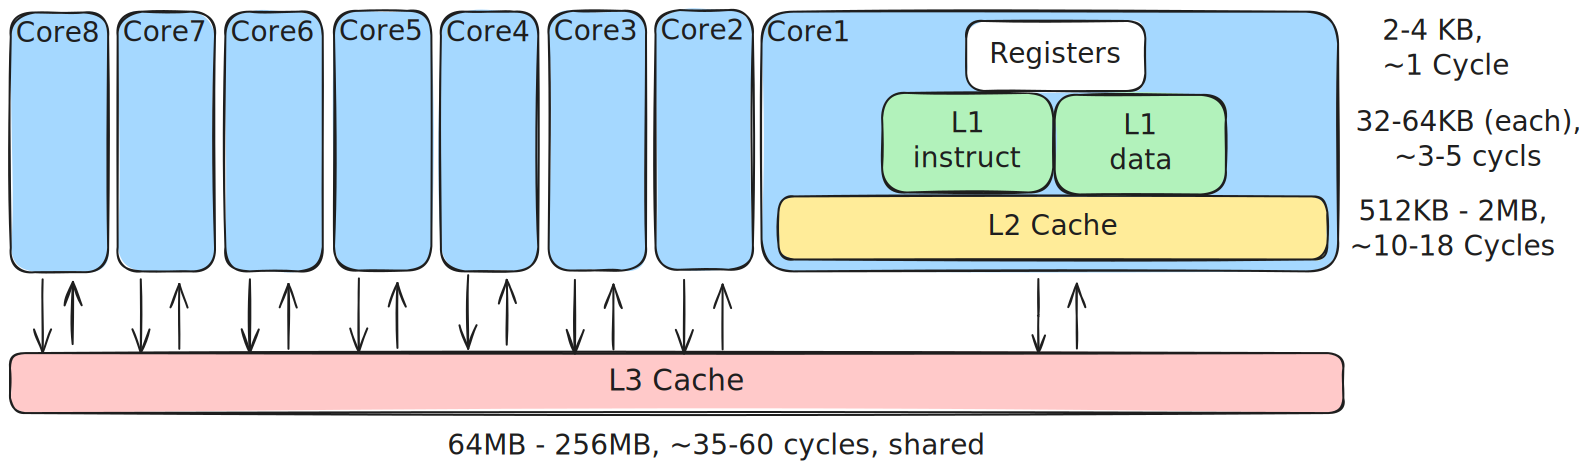
\includegraphics[width=0.65\textwidth]{CPUCacheHierarchy}
  \caption{Memory hierarchy of a modern CPU, showing the register file and cache levels (L1, L2, L3) before main memory (DRAM).}
  \label{fig:cpu-cache-hierarchy}
\end{figure}
As shown in \cref{fig:cpu-cache-hierarchy}, modern CPUs rely on a deep cache hierarchy to reduce effective memory latency.


\paragraph{GPU Memory Hierarchy}
\begin{figure}[H]
  \centering
  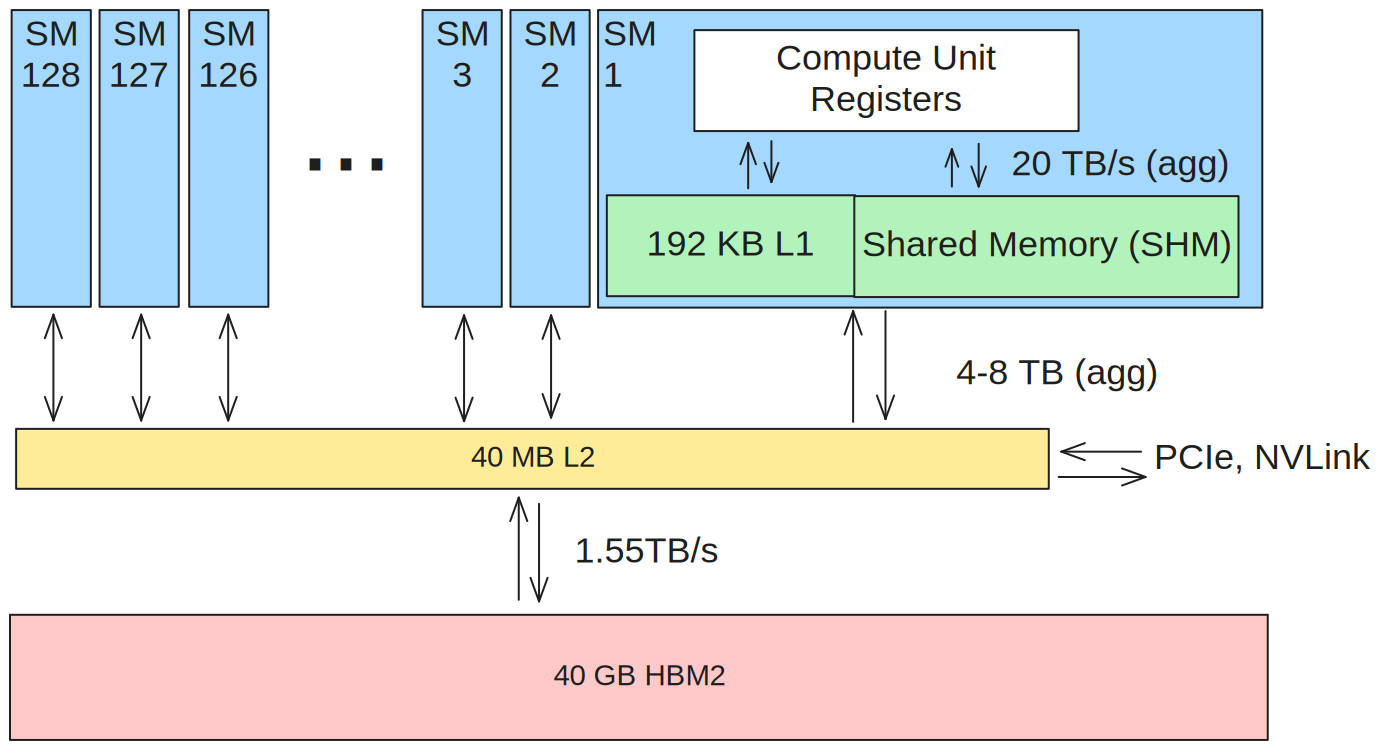
\includegraphics[width=0.65\textwidth]{A100CacheHierarchy}
  \caption{Memory hierarchy of a modern CPU, showing the register file and cache levels (L1, L2, L3) before main memory (DRAM).}
  \label{fig:a100-cache-hierarchy}
\end{figure}
In contrast to CPUs, which rely heavily on large cache hierarchies to reduce memory latency, GPUs employ a memory hierarchy designed primarily to maximise memory bandwidth and support massive parallelism. The GPU memory hierarchy consists of several levels with different capacities, latencies, and scopes, ranging from fast on-chip storage to high-capacity off-chip main memory.

At the lowest level, each thread has access to a private register file located within the Streaming Multiprocessor (SM). Registers provide the fastest storage available on the GPU, with single-cycle access latency, and are used to hold temporary variables during computation. However, registers are a limited resource and are allocated per thread, which directly affects the maximum number of concurrent threads that can reside on an SM.

The next level is shared memory, which is also located on-chip and shared among all threads within a thread block. Shared memory has significantly lower latency than global memory and much higher bandwidth, making it suitable for explicitly managed data reuse and communication between threads. Efficient use of shared memory is essential for many high-performance GPU kernels, particularly those implementing tiled matrix multiplication and tensor contraction algorithms.

Beyond shared memory, modern GPUs include a unified L2 cache shared across all SMs. The L2 cache serves to reduce the average latency of global memory accesses and to improve effective memory bandwidth by caching frequently accessed data. Unlike CPU caches, GPU caches are generally smaller relative to the number of compute units, reflecting the design emphasis on throughput rather than latency optimisation.

The main device memory of the GPU is implemented using High Bandwidth Memory (HBM), a three-dimensional stacked DRAM technology integrated on the same package as the GPU. HBM achieves extremely high memory bandwidth by using a very wide memory interface with thousands of parallel data lines, in contrast to conventional DRAM technologies that rely on narrower interfaces and higher clock frequencies. The NVIDIA A100 GPU employs HBM2e memory, providing a capacity of \SI{80}{\giga\byte} and a peak bandwidth of \SI{2039}{\giga\byte\per\second}, as shown in \cref{tab:a100-specs}.

Although HBM provides very high bandwidth, its access latency is substantially higher than that of on-chip memories such as registers and shared memory. Consequently, achieving high performance on GPUs requires structuring computations to maximise data reuse in fast on-chip memory and to access global memory in a bandwidth-efficient manner. In many scientific applications, including tensor network contractions, overall performance is often limited by the available memory bandwidth rather than by the peak floating-point throughput of the compute units.

This hierarchical organisation is summarised conceptually as follows:

\begin{itemize}
\item \textbf{Registers:} fastest storage, private to each thread, limited capacity
\item \textbf{Shared memory:} fast on-chip memory shared within a thread block
\item \textbf{L2 cache:} intermediate storage shared across all SMs
\item \textbf{HBM global memory:} large-capacity, high-bandwidth main memory
\end{itemize}

Efficient utilisation of this memory hierarchy is a central factor in the performance of GPU kernels and plays a critical role in the optimisation of tensor network algorithms.

\subsection{NVIDIA A100 Ampere Architecture}\label{sec:a100}
\subsubsection{Hardware Overview}

\begin{table}[t]
\centering
\caption{Key hardware specifications of the NVIDIA A100 (SXM4-80GB).}
\label{tab:a100-specs}
\begin{tabularx}{\textwidth}{X r}
\toprule
Property & Value \\
\midrule
Streaming Multiprocessors (SMs) & \num{108} \\
CUDA cores per SM & \num{64} \\
Tensor cores per SM & \num{4} \\
Warp schedulers per SM & \num{4} \\
Maximum threads per SM & \num{2048} \\
Maximum warps per SM & \num{64} \\
Maximum blocks per SM & \num{32} \\
Register file size per SM (32-bit registers) & \num{256000} \\
Shared memory per SM (KB) & \num{164} \\
L2 cache size (MB) & \num{40} \\
HBM memory capacity (GB) & \num{80} \\
Peak memory bandwidth (GB/s) & \num{2039} \\
Base clock frequency (GHz) & \num{1.41} \\
\bottomrule
\end{tabularx}
\end{table}

The A100 employs HBM2e as its main device memory, providing the high memory bandwidth necessary to sustain its computational throughput.

\subsubsection{Theoretical Peak Performance}

\begin{table}[t]
\centering
\caption{Theoretical peak floating-point throughput of the A100 GPU.}
\label{tab:a100-peak-performance}
\begin{tabularx}{\textwidth}{X r r}
\toprule
Precision & Peak TFLOPS & Relative speed \\
\midrule
FP64 (CUDA cores) & \num{9.7} & 1.0$\times$ \\
FP64 (Tensor cores) & \num{19.5} & 2.0$\times$ \\
FP32 & \num{19.5} & 2.0$\times$ \\
TF32 (Tensor cores) & \num{156.0} & 16.1$\times$ \\
FP16 (Tensor cores) & \num{312.0} & 32.2$\times$ \\
\bottomrule
\end{tabularx}
\end{table}


\subsubsection{Derived Performance Limits}

\begin{table}[t]
\centering
\caption{Derived theoretical limits of the A100 architecture.}
\label{tab:a100-derived}
\begin{tabularx}{\textwidth}{X r}
\toprule
Metric & Value \\
\midrule
Peak FP32 performance per SM (TFLOPS) & \num{0.18} \\
Peak FP64 performance per SM (TFLOPS) & \num{0.09} \\
Tensor core FP16 performance per SM (TFLOPS) & \num{2.89} \\
Memory bandwidth per SM (GB/s) & \num{18.88} \\
Total CUDA cores & \num{6912} \\
Total FP64 cores & \num{3456} \\
Maximum resident warps & \num{6912} \\
Maximum resident threads & \num{221184} \\
Arithmetic intensity threshold FP32 (FLOPs/byte) & \num{9.6} \\
Arithmetic intensity threshold FP64 (FLOPs/byte) & \num{4.8} \\
\bottomrule
\end{tabularx}
\end{table}


\subsubsection{Memory Latency}

\begin{table}[t]
\centering
\caption{Approximate memory access latency at different hierarchy levels.}
\label{tab:a100-memory-latency}
\begin{tabularx}{\textwidth}{X r}
\toprule
Memory level & Latency (cycles) \\
\midrule
Registers & \num{1} \\
Shared memory & \num{20} \\
L2 cache & \num{200} \\
HBM global memory & \num{500} \\
\bottomrule
\end{tabularx}
\end{table}

\section{CUDA Programming Model}\label{sec:cuda}

\subsection{Thread Hierarchy and Kernel Launch}\label{sec:cuda-threads}
\begin{figure}[H]
  \centering
  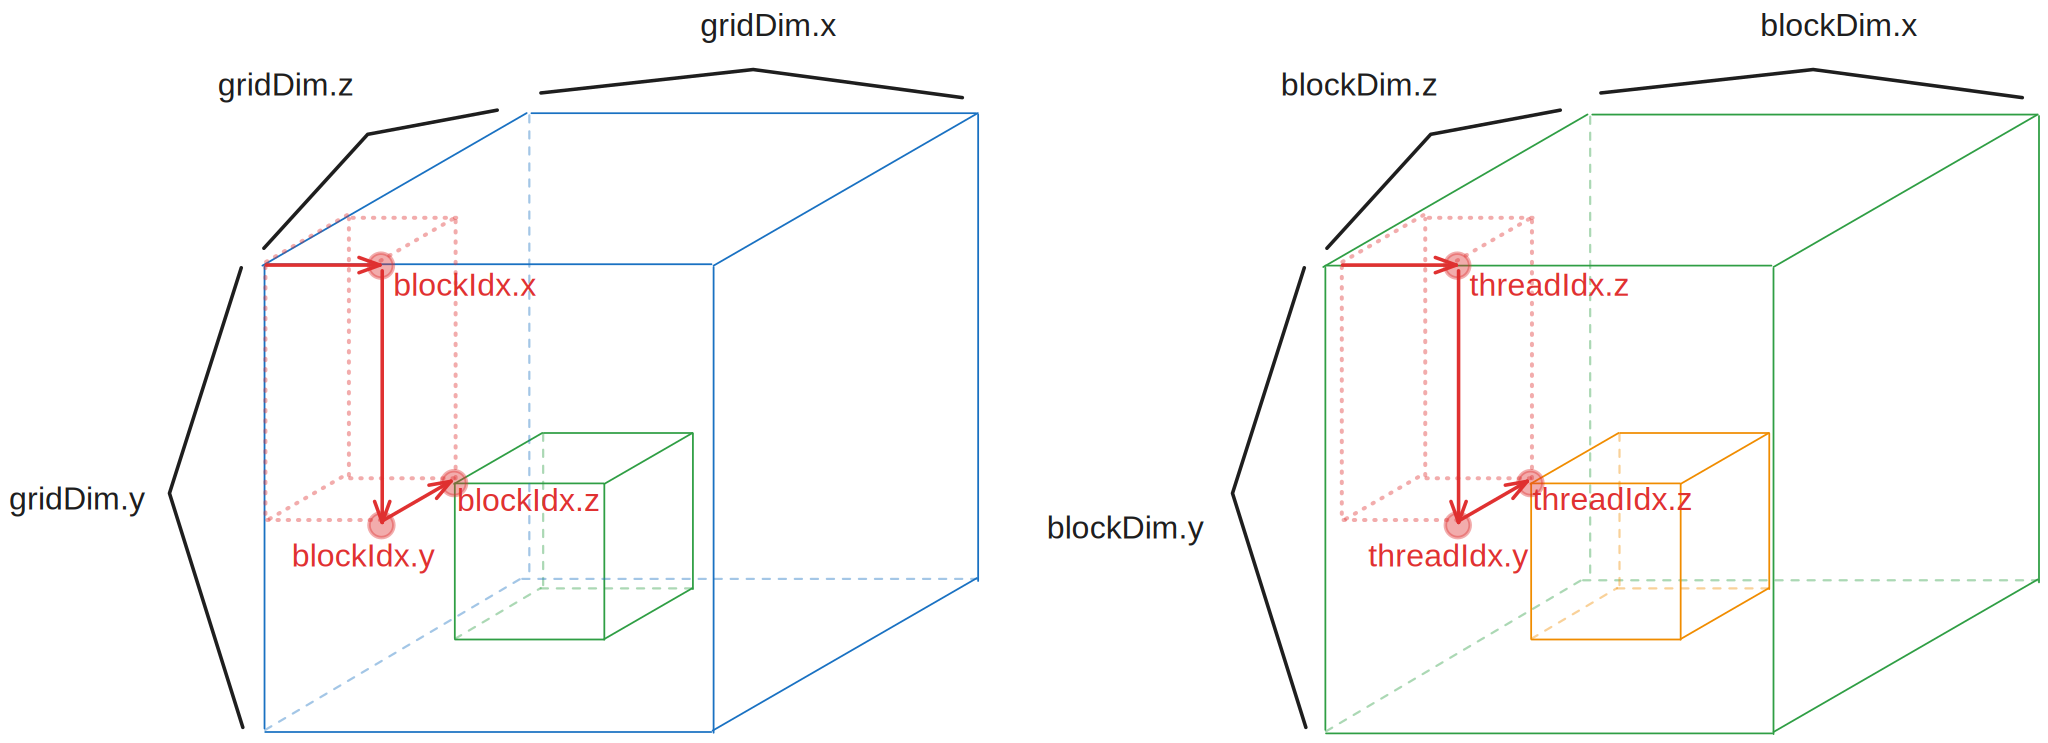
\includegraphics[width=0.85\textwidth]{GridBlockThreadAddressing}
  \caption{CUDA execution hierarchy showing the mapping of grids to thread blocks and threads. Threads are organised in up to three dimensions and identified using the built-in variables \texttt{threadIdx} and \texttt{blockIdx}.}
  \label{fig:cuda-thread-hierarchy}
\end{figure}
The hierarchical organisation of grids, thread blocks, and threads is illustrated in \cref{fig:cuda-thread-hierarchy}.

\subsection{Shared Memory and Synchronisation}\label{sec:shared-memory}

\subsection{Memory Coalescing and Bank Conflicts}\label{sec:coalescing}

\subsection{Performance Profiling with Nsight Compute}\label{sec:nsight}

\section{Related Work}\label{sec:related-work}

\subsection{cuBLAS and cuTENSOR}\label{sec:cublas-cutensor}

\subsection{ChASE Eigensolver}\label{sec:chase}

\subsection{Existing GPU Tensor Network Implementations}\label{sec:existing-tn-gpu}
